\chapter{Instruction Register}
\label{chap:instruction-reg}
This chapter gives an overview of the design and operation of Instruction Register. It contains the following sections:
\begin{itemize}
    \item \hyperref[sec:about-instruction-reg]{About Instruction Register}
    \item \hyperref[sec:design-instruction-reg]{Design of Instruction Register}
    \item \hyperref[sec:operation-instruction-reg]{Operational Overview}
    \item \hyperref[sec:instruction-decoder]{Instruction Decoder}
\end{itemize}

\newpage

\section{About Instruction Register}
\label{sec:about-instruction-reg}
The instruction register allows an instruction to be shifted into the design. The instruction is used to select the test to be performed or the test data register to be accessed or both. Also, store JTAG instructions for instruction decoder.

\section{Design of Instruction Register}
\label{sec:design-instruction-reg}
The purpose of Instruction Register is to shift in instruction through TDI and having the provision to store the instruction till a new instruction is fully shifted in. Typically an IR has two registers inside it as shown below. The Hold Register stores the previous instruction and the Shift Register is used to shift-in the next instruction without affecting the previous instruction’s execution. 

\vspace{1cm}
\begin{figure}[H]
    \centering
    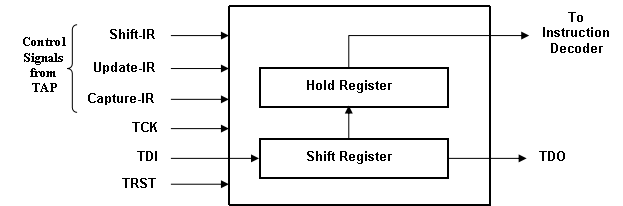
\includegraphics[width = 12cm]{images/instruction_register_top.png}
    \vspace{1cm}
    \caption{Top Level View of Instruction Register}
    \label{fig:instruction-reg-top}
\end{figure}
\vspace{1cm}

The instruction shifted into the instruction register shall be latched such that \linebreak changes in the effect of an instruction occur only in the Update-IR and Test-Logic-Reset TAP controller states.

\vspace{1cm}
\begin{figure}[H]
    \centering
    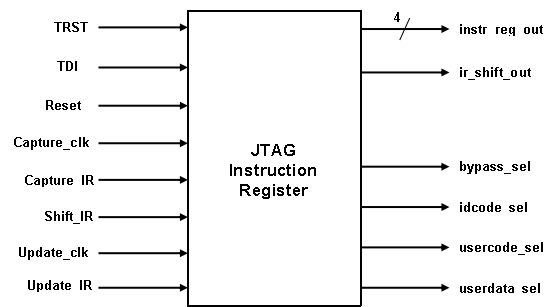
\includegraphics[width = 10cm]{images/jtag_instruction_register.png}
    \vspace{1cm}
    \caption{JTAG Instruction Register}
    \label{fig:jtag-instruction-reg}
\end{figure}
\vspace{1cm}

The control signals to the Instruction register originates from the TAP controller and depending upon the FSM state can either cause a shift-in/shift-out through the Shift Register (serial update operation in Shift-IR state ), or cause the contents of the Shift Register to be passed across to the Hold Register (parallel update operation in Update-IR state). 

\subsection{Instruction Register Ports}

\begin{longtable}{l l p{9.5cm}}
    \caption{Instruction Register port description}
    \label{tab:instruction-reg-ports}\\
    \hline
         \textbf{Port Name} & \textbf{Direction} & \textbf{Description}\\ \hline \hline
        \hyperref[subsec:trst]{TRST} & Input & Asynchronous Active low reset: If asserted default IDCODE Instruction is selected. \\ \hline
        \hyperref[subsec:tdi]{TDI} & Input & Test Data Input \\ \hline
        Reset & Input & Asserted when the state is in the TEST\_LOGIC\_RESET state. During the posedge of Update\_clk if asserted default IDCODE instruction is selected. \\ \hline
        Capture\_clk & Input & Capture\_clk (posedge of TCK) captures the instruction. \\ \hline
        Capture\_IR & Input & Controls the Capture Operations, captures the instruction during Capture\_IR stage in the posedge of Capture\_clk if no TRST and Reset is there. Basically it captures 4’b0001 instructions when Capture\_IR is asserted. The JTAG standard requires the last two bits ‘01’. \\ \hline
        Shift\_IR & Input & Controls the Shift Operation, Shifts the TDI bit during the posedge of Capture\_clk from one cell to other cell. \\ \hline
        Update\_clk & Input & Update\_clk (negedge of TCK) updates the instruction. \\ \hline
        Update\_IR & Input & Controls the Update\_IR Operations, during the posedge of Update\_clk if no TRST and Reset then Shift Stage instructions are updated to instr\_reg\_out. \\ \hline
        instr\_reg\_out & Output & Instruction register output gets the instruction to be performed by JTAG. \\ \hline
        ir\_shift\_out & Output & 1-bit instruction bit shifted out during Shift\_IR operation Stage. \\ \hline
        bypass\_sel & Output & BYPASS Instruction is executed, if
        
        \texttt{instr\_reg\_out = 4’hF}. \\ \hline
        idcode\_sel & Output & IDCODE Instruction is executed, If
        
        \texttt{instr\_reg\_out = 4’h2}. \\ \hline
        usercode\_sel & Output & USER\_CODE Instruction is executed, if
        
        \texttt{instr\_reg\_out = 4’h6}. \\ \hline
        userdata\_sel & Output & USER\_DATA Instruction is executed, if
        
        \texttt{instr\_reg\_out = 4’h8}. \\ \hline
\end{longtable}

\newpage

\section{Operational Overview}
\label{sec:operation-instruction-reg}
All operations of shift-register stages shall occur on the rising edge of TCK after entry into a controller state.

\begin{enumerate}
    \item The clock input (Clock-IR) to the register in the serial path is applied only during the Capture-IR and Shift-IR TAP controller states.
    \item The data present at the parallel output of the instruction register shall be latched from the shift-register stage on the falling edge of TCK in the Update-IR controller state. The clock input (Update-IR) to the hold register is applied only during the Update-IR TAP controller state.
    \item The parallel output (labeled Instruction bit) is updated at the end of the \linebreak instruction-scan cycle during the Update-IR controller state.
    \item The parallel output is reset in the Test-Logic-Reset controller state as a result of a logic 0 received at the Reset input of the cell. After entry into the Test-Logic-Reset controller state as a result of the clocked operation of the TAP controller, the IDCODE instruction (or, if there is no device identification register, the BYPASS instruction) shall be latched onto the instruction register output on the falling edge of TCK.
    \item If the TRST input is provided and a low signal is applied to the input, the latched instruction shall change asynchronously to IDCODE (or, if no device identification register is provided, to BYPASS).
    \item JTAG standard requires the last two bits of parallel load = ‘01’ which is closest to TDO and Scan operation does not interfere with instruction decoder.
\end{enumerate}

\vspace{0.5cm}
\begin{figure}[H]
    \centering
    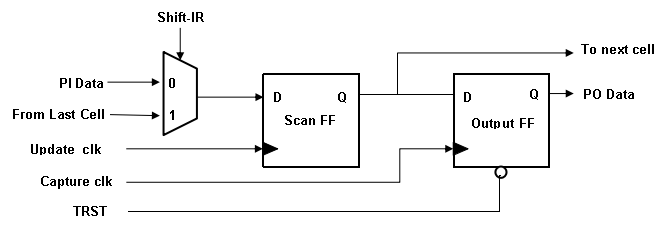
\includegraphics[width = 15cm]{images/instruction_register_cell.png}
    \vspace{1cm}
    \caption{Instruction Register Cell}
    \label{fig:instruction-reg-cell}
\end{figure}

\newpage

\section{Instruction Decoder}
\label{sec:instruction-decoder}
The instruction from the Instruction Register (IR) is fed to a decoder logic, which selects the Data Register for JTAG operation. We assign a unique value (or opcode) to each and every Data Register in the JTAG. In order to select a Data Register, we load the IR with the corresponding opcode and the Instruction Decoder decodes the value and establishes an access path between the TDI/TDO and the required Data Register.

\vspace{1cm}
\begin{figure}[H]
    \centering
    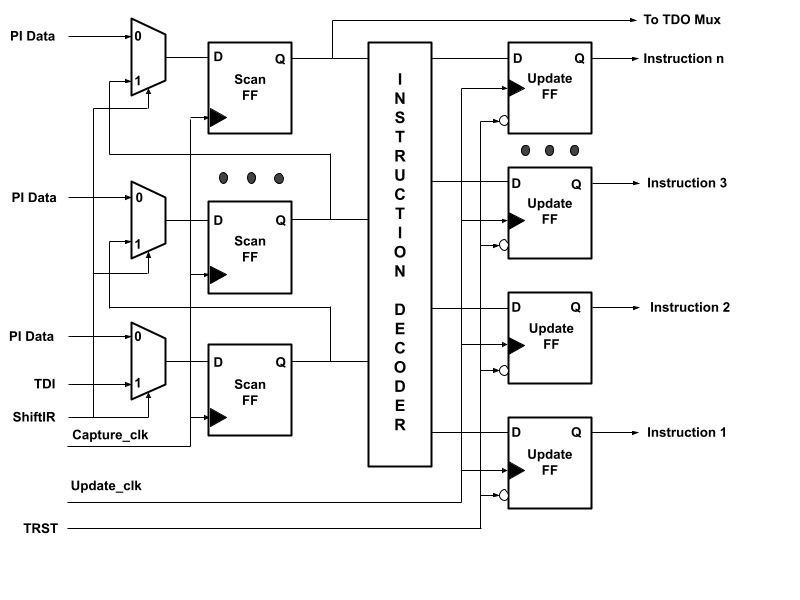
\includegraphics[width = 15cm]{images/instruction_register_shift_update.png}
    \vspace{1cm}
    \caption{Instruction decoder between shift and update stages}
    \label{fig:instruction-decoder}
\end{figure}
\vspace{1cm}

The advantage is that the instruction decodes are now updated by a clock and are therefore glitch-free. The number of update flops or latches is now the same as the number of instructions, not the number of instruction register bits. Note that “Instruction 1” is set “on” by the “Reset” signal; this would be the mandatory BYPASS or IDCODE instruction decode.
